\begin{frame}{Going further (1): Branches}
  \begin{itemize}
    \item several people can work at the same project at the same time
    \item they might make incompatible changes (that can be united later)
    \item git allows the versions of a repository to diverge using branches
    \inote{they can also be brought back together using merging later}
    \item The default branch is usually called ``master''
    \item Each branch has a so-called HEAD that points to its latest commit
    \item There is also a HEAD of the repository which points to the current branch
  \end{itemize}
\end{frame}

\begin{frame}{Going further (2): Branching \& Merging}
  \begin{columns}[onlytextwidth]
    \begin{column}{0.5\textwidth}
      \begin{itemize}
        \item you can make commands on branches like you would normally
        \inote{but you need to switch to the branch first}
        \begin{itemize}
          \item \shellcmd{git branch name} - create a branch
          \item \shellcmd{git checkout name} - switch to it
          \item \shellcmd{git merge name} - merge a branch back into the current one
        \end{itemize}
      \end{itemize}
    \end{column}
    \begin{column}{0.5\textwidth}
      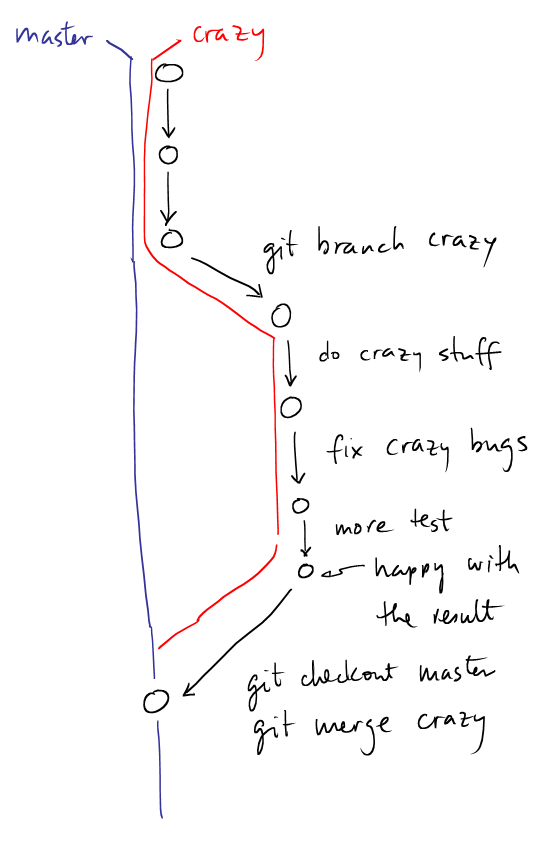
\includegraphics[height=\textheight]{imgs/branches}
    \end{column}
  \end{columns}
\end{frame}

\begin{frame}{Going further (3): Resolving Merge conflicts}
  \begin{itemize}
    \item merging can cause conflicts
    \inote{when files were modified on both branches and git can not merge them automatically}
    \item git will tell you when you run \shellcmd{git merge} if there are conflicts
    \begin{itemize}
      \item you can edit the affected files manually, then stage the files (\shellcmd{git add}) and commit them (\shellcmd{git commit})
      \inote{\shellcmd{git status} is always helpful when doing this}
      \item \shellcmd{git merge --abort} - cancel the merge and go back to what was there before
      \item ``fake'' a merge by forcing git to use one of the two versions
      \begin{itemize}
        \item \shellcmd{git merge -X ours branch} - use the version of the current branch
        \item \shellcmd{git merge -X theirs branch} - use the other branches version
        \item (you need to do this before starting to merge)
      \end{itemize}
    \end{itemize}
  \end{itemize}
\end{frame}